\chapter{Task 3}
\label{chapter:task3}
In this chapter the radiation and far field patterns  in the H- and E-plane were computed in [dBi] as a function of  the far field and observation angles in MATLAB. These patterns are useful to construct so that the radiation adn far field functions from the antenna can be better understood. The radiation pattern is  defined as the variation of radiated power by an antenna as a function of the direction from the antenna, the pattern is one of the quantities that are observed in the antenna's far field region
which gives us the freedom to fully utilize the theory regarding the far field region and Fraunhofer approximation.

The theory is first presented in the section below and then the results from the simulations are presented in section \ref{chapter3:results}.


\section{Theory}
For the horizontal dipole which is directed in the y direction the H-plane lies in the plane which corresponds to $\phi =0$. The E-plane then must lie in the plane which has $\phi = \pi/2$, as the E-field  is perpendicular to the H-field. With this knowledge it is easy to plot the radiation pattern for the co polarization according to the function 
\begin{equation}
Pattern = 10\cdot~^{10}log\left(\frac{4\pi |G_{co}(\theta, \phi_0)|^2}{P_{rad}2\eta} \right).
\end{equation}
Here the co polar radiation pattern is only considered, and is has also been normalized with respect to the radiated power. By taking the logarithm of the pattern the results will be given in [dBi] which is commonly used in antenna theory.

The far field patterns for the E- and H-plane of the far field function are defined as $|G_{co}(\theta , 0)|$ and $|G_{co}(\theta , pi/2)|$ in the H- and E- planes respectively. These patterns can be plotted in dBi as 
\begin{equation}
Pattern = 10 \cdot ~^{10}log\left(\frac{4\pi |G_{co}(\theta, \phi_0)|}{\sqrt{P_{rad}2\eta}} \right).
\end{equation}
\cite{kildal2000foundations}


\section{Results}
\label{chapter3:results}
The MATLAB code for this task can be viewed in appendix \ref{section:task3.m}. The result for the co polarization radiation pattern in the E- and H-plane was plotted in figure \ref{task3:E-plane} and \ref{task3:H-plane}, respectively.

\begin{figure}[h]
\centering
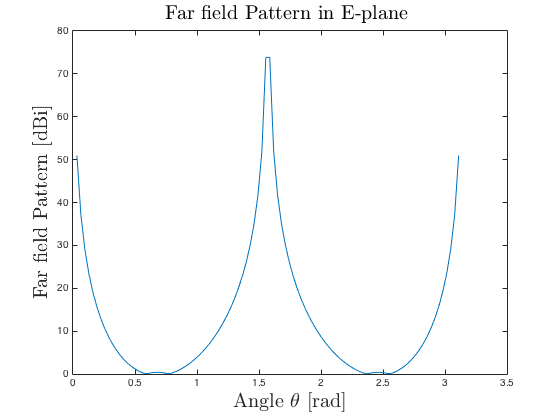
\includegraphics[scale=0.35]{/Users/marikasvensson/Documents/MATLAB/MicroProject/finished/task3/Eplane.png}
\caption{This figure shows the radiation pattern in the E-plane}
\label{task3:E-plane}
\end{figure}


\begin{figure}[h]
\centering
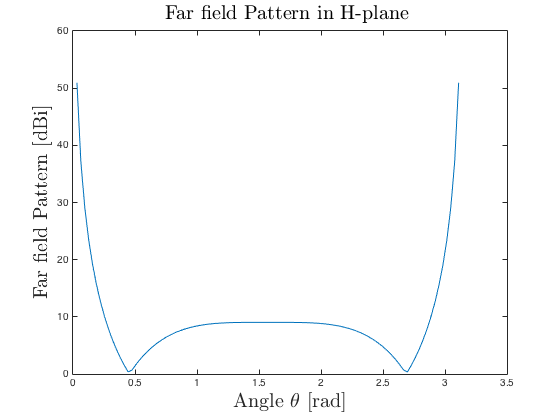
\includegraphics[scale=0.35]{/Users/marikasvensson/Documents/MATLAB/MicroProject/finished/task3/Hplane.png}
\caption{This figure shows the radiation pattern in the H-plane}
\label{task3:H-plane}
\end{figure}

The patterns of the far field function were plotted in figures \ref{task3:PatternE-plane} and \ref{task3:PatternE-plane} for the E- and H-plane. 

\begin{figure}[h]
\centering
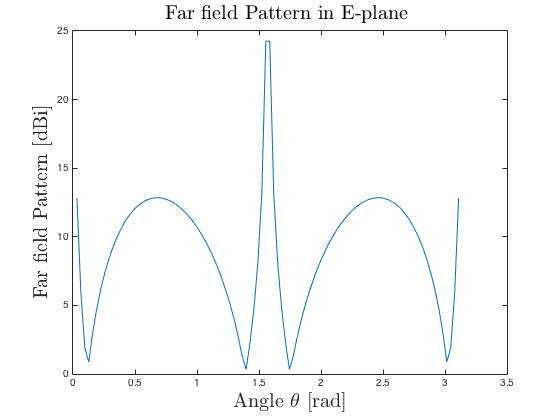
\includegraphics[scale=0.35]{/Users/marikasvensson/Documents/MATLAB/MicroProject/finished/task3/PatternEplane.png}
\caption{This figure shows the far field pattern in the E-plane}
\label{task3:PatternE-plane}
\end{figure}


\begin{figure}[h]
\centering
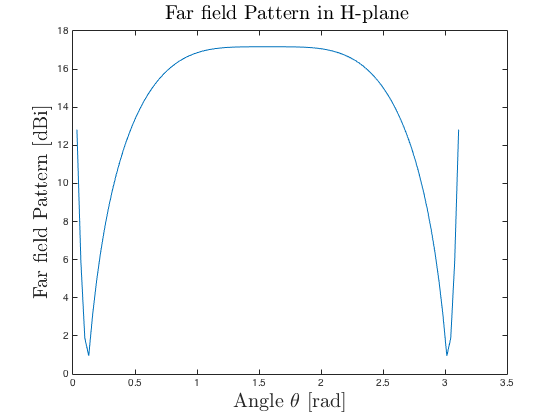
\includegraphics[scale=0.35]{/Users/marikasvensson/Documents/MATLAB/MicroProject/finished/task3/PatternHplane.png}
\caption{This figure shows the far field pattern in the H-plane}
\label{task3:PatternH-plane}
\end{figure}


